\section{Aufgabenstellung und Versuch}

Aus den bereits aufgestellten DGL-System kann das Blockschaltbild in Simulink
erstellt werden.

\begin{figure}[H]
    \centering
    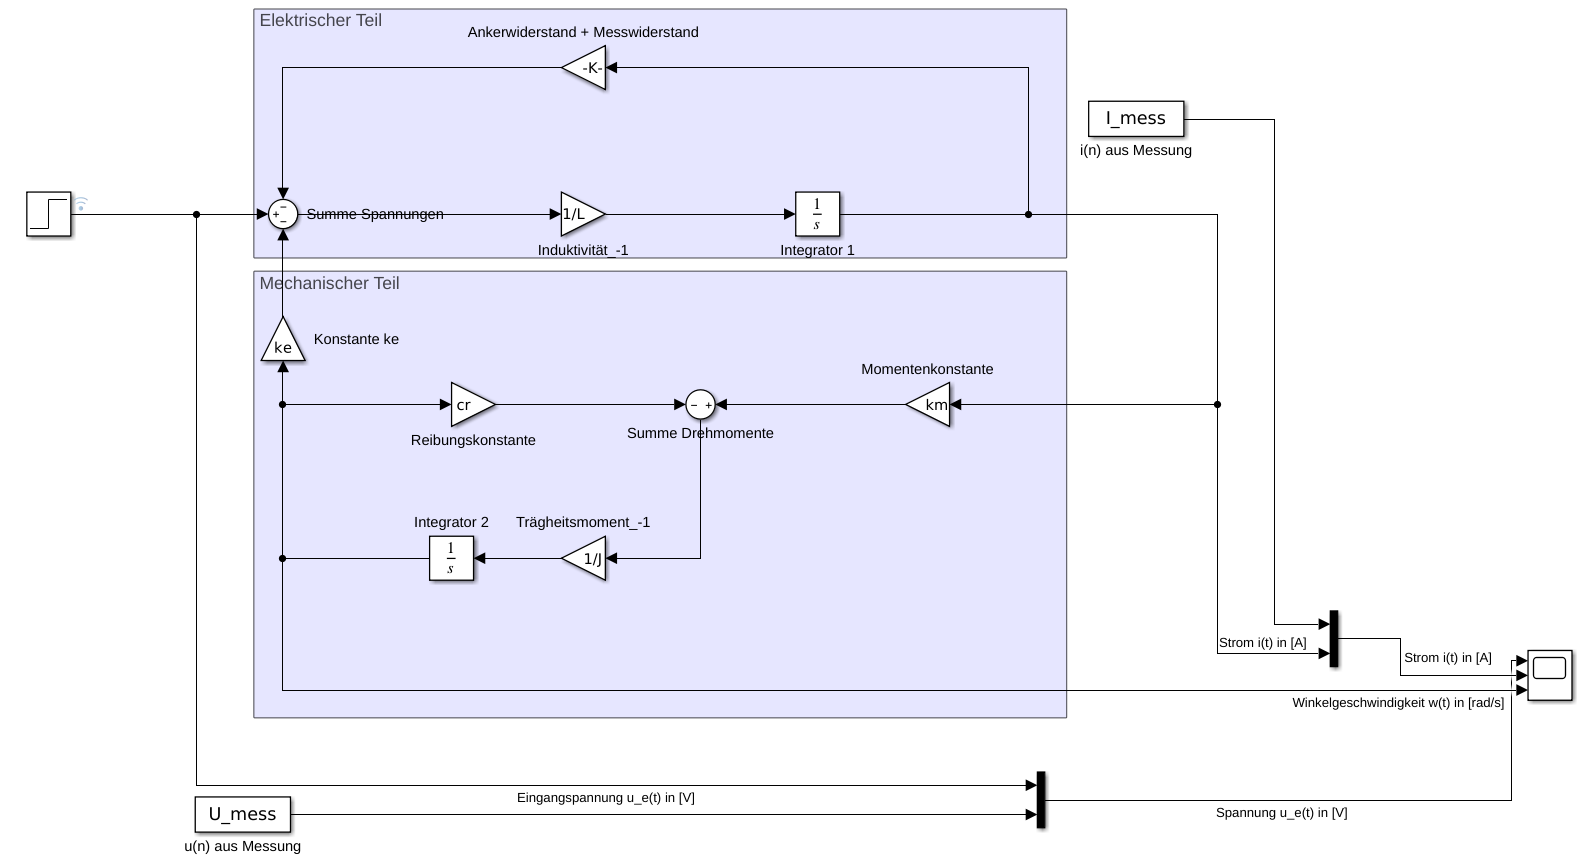
\includegraphics[width=1\textwidth]{sl_modell.png}
    \caption{Blockschaltbild in Simulink}
    \label{fig:Blockschaltbild}
\end{figure}

Als Eingang wurde ein Step-Block benutzt und als Ausgang Scope-Block.
Die erste DGL wurden im oberen Teil des Modell realisiert und beschreibt
den elektrischen Teil des Systems. Im unteren wird der mechanische Teil
des Motors modelliert der aus der zweiten DGL hervorgeht.\\

Die Konstanten wurden in einem Matlab-File abgespeichert und werden über
dieses auch aufgerufen. Auch die Daten der Messung des Spungs und der
Sprungantwort sind hier zufinden.\\

Um den gemessenen Spung und die Sprungantwort in Simulink anzuzeigen wurde der Block
"From Workspace" benutzt der jeweils den Zeit-Spannungs-Vektor und den Zeit-
Spannungs-Vektor lädt.

Der Spung auf das Modell wurden dem Sprung aus der Messung angepasst.

STEPTIME 0.048s
FINAL VALUE 8.2V
SAMPLETIME 0.001s
